%!TeX root=./torneio.tex

\FloatBarrier

\subsection{Inserção e remoção em torneio} \label{subsec:torneio-insere-remove}

Assim como fizemos na Seção~\ref{sec:abb}, além das operações
\textsc{advance}$(t)$, \textsc{change}$(j, v)$ e
\textsc{query\_max}$()$, poderíamos querer dar suporte a operações
como:

\begin{itemize}
    \item \textsc{insert}$(v, x_t)\rightarrow$ insere um elemento
    com velocidade $v$ e valor $x_t$ no instante \now;
    \item \textsc{delete}$(i) \rightarrow$ remove o elemento $i$ no
    instante \now.
\end{itemize}
Agora, diferentemente da Seção~\ref{sec:abb}, não utilizaremos uma nova estrutura para dar suporte
a essas operações, pois um torneio já suporta operações como inserção e remoção de elementos em
tempo logarítmico.
Porém, da maneira como se encontra a interface, poderíamos ter problemas como espaços de memória
ociosos após várias remoções ou um gasto elevado de tempo redimensionando vetores para que
suportem a inserção de novos elementos.
Dessa forma, descreveremos a seguir alterações a serem feitas na interface para evitar problemas
como os citados.

Inicialmente o vetor que guarda o torneio começa com os elementos ocupando as suas últimas
posições e construímos o torneio de acordo com o valor de cada elemento no instante $t = 0$.

Uma vez montado o torneio, construímos um certificado para cada elemento no torneio.
Agora os certificados não serão mais mantidos em um vetor;
serão mantidos junto aos elementos para facilitar a inserção e remoção de certificados, já que
estas vêm junto com a inserção e remoção de elementos.
O certificado de um elemento $e$ se refere à relação estabelecida entre o elemento $e$ e o
elemento $k$, que é o elemento que venceu $e$ na última partida que $e$ disputou, e consiste no
instante de tempo em que o elemento $e$ passará a ter um valor maior que o valor do elemento $k$,
se esse instante for maior que o instante atual.
Do contrário, o certificado consiste em $+\infty$.

Note que o elemento que está na primeira posição do torneio não é vencido por ninguém no instante
\now.
Portanto, daremos o valor $+\infty$ para o seu certificado.

Esses $n$ certificados serão colocados em uma fila com prioridades, com o prazo de validade como
prioridade.
O certificado com menor prazo de validade estará ocupando a primeira posição da fila.
Na verdade, como os certificados estarão diretamente ligados aos elementos, colocaremos os
elementos nessa fila.

Para descrever as implementações das operações \textsc{advance}$(t)$, \textsc{change}$(j, v)$,
\textsc{query\_max}$()$, \textsc{insert}$(v, x_t)$ e \textsc{delete}$(i)$, vamos estabelecer os
nomes dos objetos, variáveis e rotinas auxiliares utilizados:
\begin{enumerate}
    \item $n$: número de elementos no instante \now;
    \item \elemento: elemento com os seguintes atributos:
    \begin{enumerate}
        \item \id: atributo para identificar o elemento.
        Daqui em diante, usaremos elemento $i$ para se referir ao elemento
        cujo \id~é $i$;

        \item \speed: a velocidade do elemento;

        \item \initv: é o valor que o elemento possuía no
        instante $t = 0$;

        \item \cert: o prazo de validade do certificado do
        elemento;

        \item \pqpos: posição do elemento
        na fila com prioridades $Q$;

        \item \lastmatch: posição do
        vetor \torneio~em que o elemento disputou sua última
        partida.
        É o equivalente do vetor $\textit{indT}$.
    \end{enumerate}
    \item \torneio: vetor, de $2n - 1$ posições, que guarda
    apontadores para os elementos formando um torneio de acordo com
    seus valores no instante \now;

    \item \Q: fila com prioridades que contém os elementos, com o
    elemento com certificado de menor valor à frente;

    \item \textsc{insertTourn}$(e) \rightarrow$ insere $e$, que é um
    elemento, no torneio armazenado em $\torneio$ e atualiza os certificados necessários no
    processo;

    \item \textsc{deleteTourn}$(e) \rightarrow$ remove $e$, que é um
    elemento, do torneio armazenado em $\torneio$ e atualiza os certificados necessários no
    processo.
\end{enumerate}
Para a implementação das operações \textsc{change}$(j, v)$ e \textsc{delete}$(i)$, precisamos de
alguma maneira recuperar um elemento baseado no seu \id.
Para tal, podemos utilizar uma tabela de símbolos.
A seguir~estão três operações que nos ajudarão a recuperar os elementos:
\begin{enumerate}
    \item \textsc{getObject}$(i)\rightarrow$ retorna o elemento $i$;
    \item \textsc{insertObject}$(e) \rightarrow$ insere $e$, que é
    um elemento, na tabela de símbolos;
    \item \textsc{deleteObject}$(e) \rightarrow$ remove $e$, que é
    um elemento, da tabela de símbolos.
\end{enumerate}
Para permitir a inserção e remoção de certificados, a interface da fila com prioridades será
reformulada, contando com duas operações extras:
\begin{enumerate}
    \item \textsc{insertPQ}$(Q, e) \rightarrow$ insere $e$ na fila
    com prioridades $Q$;
    \item \textsc{deletePQ}$(Q, e) \rightarrow$ remove $e$ da fila
    com prioridades $Q$;
    \item \textsc{updatePQ}$(Q,e,t) \rightarrow$ muda o valor do
    certificado de $e$ para $t$ e atualiza a fila com prioridades
    $Q$;
    \item \textsc{minPQ}$(Q) \rightarrow$ devolve o elemento com o
    certificado de menor valor da fila com prioridades $Q$.
\end{enumerate}
As operações \textsc{updatePQ}$(Q,e,t)$ e \textsc{deletePQ}$(Q, e)$ podem ser implementadas em
tempo logarítmico no número de elementos em $Q$ graças ao atributo \pqpos~dos elementos.

Um evento está associado a um certificado $(e, t)$ que expira no instante $t$.
As implementações das operações \textsc{event}, \textsc{query\_max} e \textsc{change} são
similares às implementações da Seção~\ref{sec:torneio}.

\begin{figure}[H]
    \centering
    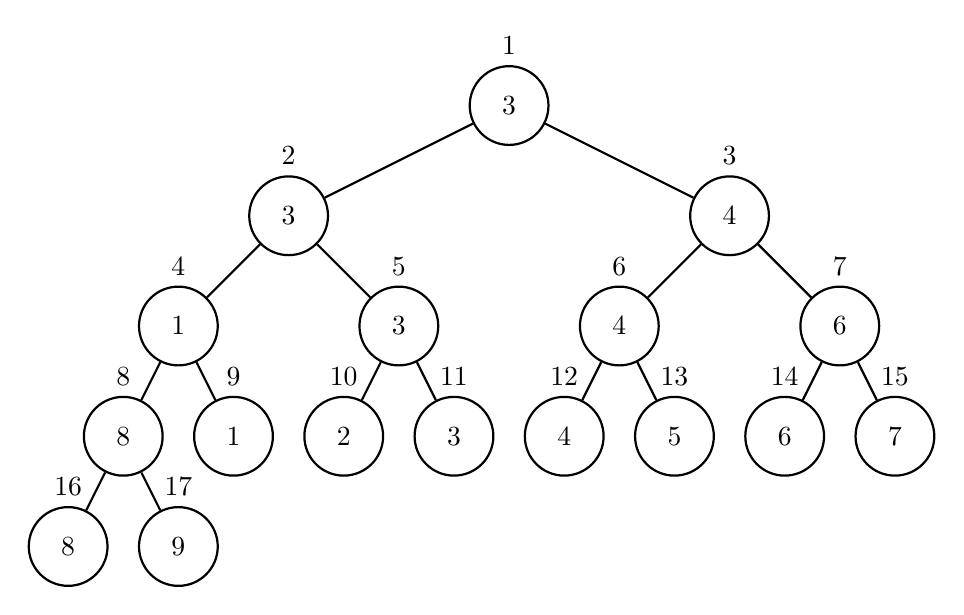
\begin{tikzpicture}[thick, scale=0.7]
        \node[label={1},circle,draw,minimum size=1cm]
        (1) at (0,0) {$3$};
        \node[label={2},circle,draw,minimum size=1cm]
        (2) at (-4,-2) {$3$};
        \node[label={3},circle,draw,minimum size=1cm]
        (3) at (4,-2) {$4$};
        \node[label={4},circle,draw,minimum size=1cm]
        (4) at (-6,-4) {$1$};
        \node[label={5},circle,draw,minimum size=1cm]
        (5) at (-2,-4) {$3$};
        \node[label={6},circle,draw,minimum size=1cm]
        (6) at (2,-4) {$4$};
        \node[label={7},circle,draw,minimum size=1cm]
        (7) at (6,-4) {$6$};
        \node[label={8},circle,draw,minimum size=1cm]
        (8) at (-7,-6) {$8$};
        \node[label={9},circle,draw,minimum size=1cm]
        (9) at (-5,-6) {$1$};
        \node[label={10},circle,draw,minimum size=1cm]
        (10) at (-3,-6) {$2$};
        \node[label={11},circle,draw,minimum size=1cm]
        (11) at (-1,-6) {$3$};
        \node[label={12},circle,draw,minimum size=1cm]
        (12) at (1,-6) {$4$};
        \node[label={13},circle,draw,minimum size=1cm]
        (13) at (3,-6) {$5$};
        \node[label={14},circle,draw,minimum size=1cm]
        (14) at (5,-6) {$6$};
        \node[label={15},circle,draw,minimum size=1cm]
        (15) at (7,-6) {$7$};
        \node[label={16},circle,draw,minimum size=1cm]
        (16) at (-8,-8) {$8$};
        \node[label={17},circle,draw,minimum size=1cm]
        (17) at (-6,-8) {$9$};

        \draw[thick] (1) -- (2);
        \draw[thick] (2) -- (4);
        \draw[thick] (4) -- (8);
        \draw[thick] (4) -- (9);
        \draw[thick] (8) -- (16);
        \draw[thick] (8) -- (17);
        \draw[thick] (2) -- (5);
        \draw[thick] (5) -- (10);
        \draw[thick] (5) -- (11);
        \draw[thick] (1) -- (3);
        \draw[thick] (3) -- (6);
        \draw[thick] (3) -- (7);
        \draw[thick] (6) -- (12);
        \draw[thick] (6) -- (13);
        \draw[thick] (7) -- (14);
        \draw[thick] (7) -- (15);
    \end{tikzpicture}
    \caption[Representação da estrutura torneio]{Torneio com $9$
        elementos em que $3$ é o elemento com valor máximo.}
    \label{fig:torneio:exemplo}
\end{figure}

A operação \textsc{insert}$(v, x_t)$, no Algoritmo~\ref{alg:torneioi:insert}, consiste em criar um
novo elemento, inicializando seus atributos com os devidos valores, inseri-lo no torneio e na
estrutura que usamos para recuperá-lo, calcular o seu certificado e inseri-lo na fila de
prioridade.
Lembre-se que se \now~$\neq 0$, então $x_t \neq$~\initv.
Para calcular \initv, utilizamos novamente a relação $x_t = now\cdot speed + x_0 \Rightarrow x_0 =
x_t - speed\cdot\now$.
A rotina \textsc{insertTourn} é explicada a seguir.
Veja o exemplo da Figura~\ref{fig:torneioi:insert}.

\begin{figure}[H]
    \centering
    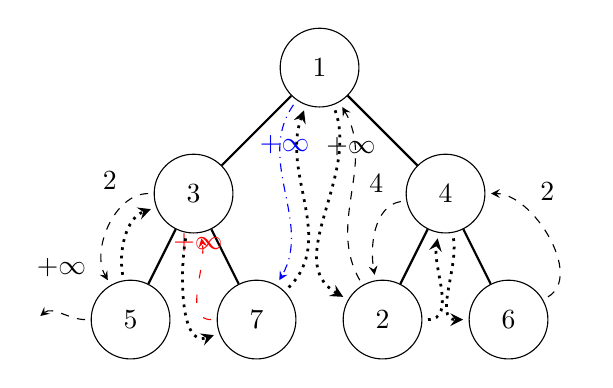
\begin{tikzpicture}[baseline=-2cm,scale=0.8]
        \node[circle,draw,minimum size=1cm] (1) at (0,0)  {$1$};
        \node[circle,draw,minimum size=1cm] (2) at (-2,-2){$3$};
        \node[circle,draw,minimum size=1cm] (3) at (2,-2) {$4$};
        \node[circle,draw,minimum size=1cm] (4) at (-3,-4){$5$};
        \node[circle,draw,minimum size=1cm] (5) at (1,-4) {$2$};
        \node[circle,draw,minimum size=1cm] (6) at (3,-4) {$6$};
        \node[circle,draw,minimum size=1cm] (7) at (-1,-4){$7$};
        % \node[label={7},circle,draw,minimum size=1cm] (7) at (3,-4) {$8$};
        % \node[label={9},circle,draw,minimum size=1cm] (9) at (-2,-6) {$1$};
        \tikzstyle{filho}=[thick]
        \tikzstyle{pred}=[->, shorten >= 2pt, shorten <= 2pt,
        dashed, >=stealth]
        \tikzstyle{sucessor}=[->, shorten >= 2pt, shorten <= 2pt,
        dotted, >=stealth, line width=0.35mm]
        % \tikzstyle{p4}=[->, shorten >= 2pt, shorten <= 2pt, dotted, >=stealth]
        \draw[filho] (1) -- (2);
        \draw[filho] (1) -- (3);
        \draw[filho] (2) -- (4);
        \draw[filho] (2) -- (7);
        \draw[filho] (3) -- (5);
        \draw[filho] (3) -- (6);
        \draw[pred] (6) edge[out=30,in=0]
        node[above=10pt] {$2$} (3);
        \draw[sucessor] (3) edge[out=280,in=180] (6);
        \draw[pred] (3) edge[out=190,in=100]
        node[above=10pt] {$4$} (5);
        \draw[sucessor] (5) edge[out=0,in=260] (3);
        \draw[pred] (5) edge[out=120,in=300]
        node[above=10pt] {$+\infty$} (1);
        \draw[sucessor] (1) edge[out=290,in=150] (5);
        \draw[pred, loosely dashed, red] (7) edge[out=180,in=280]
        node[red, above=10pt] {$+\infty$} (2);
        \draw[sucessor] (2) edge[out=260,in=200] (7);
        \draw[pred, blue, dashdotted] (1) edge[out=235,in=60]
        node[blue, above=10pt] {$+\infty$} (7);
        \draw[sucessor] (7) edge[out=45,in=250] (1);
        \draw[pred] (2) edge[out=180,in=120]
        node[above=10pt] {$2$} (4);
        \draw[sucessor] (4) edge[out=100,in=200] (2);
        \draw[pred] (4) edge[out=180,in=40]
        node[above=10pt] {$+\infty$} (-4.5, -4);
    \end{tikzpicture}
    \begin{tabular}{|c|c|c|c|c|}
        \hline
        &       &       & $\now = 1$                  \\
        $i$ & $x_0$ & $v$   & $\cert[i]$                  \\
        \hline
        $1$ & $6$   & $2$   & \textcolor{blue}{$+\infty$} \\

        $2$ & $3$   & $5$   & $+\infty$                   \\

        $3$ & $2$   & $1$   & $2$                         \\

        $4$ & $7$   & $4$   & $4$                         \\

        $5$ & $-2$  & $3$   & $+\infty$                   \\

        $6$ & $14$  & $0.5$ & $2$                         \\

        $7$ & $3$   & $1$   & \textcolor{red}{$+\infty$}  \\
        \hline
    \end{tabular}
    \caption[ABB após chamar \textsc{insert}]{Após chamar
        {\normalfont \textsc{insert}$(1, 4)$}, no instante $1$, o elemento $7$ foi
    inserido na árvore.
    O certificado do elemento $7$ foi criado e o
    certificado do seu sucessor, o elemento $1$, atualizado.}
    \label{fig:abb:insert}
\end{figure}

\begin{figure}[H]
    \centering
    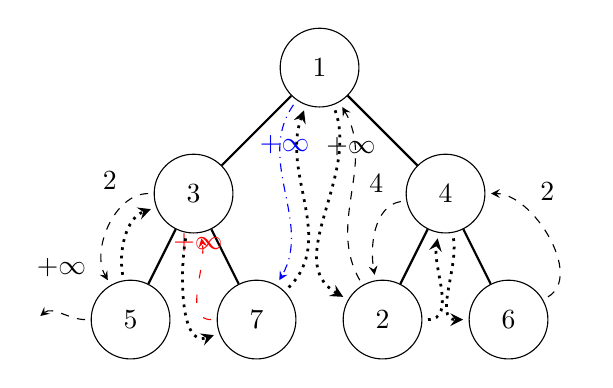
\begin{tikzpicture}[baseline=-2cm,scale=0.8]
        \node[circle,draw,minimum size=1cm] (1) at (0,0)  {$1$};
        \node[circle,draw,minimum size=1cm] (2) at (-2,-2){$3$};
        \node[circle,draw,minimum size=1cm] (3) at (2,-2) {$4$};
        \node[circle,draw,minimum size=1cm] (4) at (-3,-4){$5$};
        \node[circle,draw,minimum size=1cm] (5) at (1,-4) {$2$};
        \node[circle,draw,minimum size=1cm] (6) at (3,-4) {$6$};
        \node[circle,draw,minimum size=1cm] (7) at (-1,-4){$7$};
        % \node[label={7},circle,draw,minimum size=1cm] (7) at (3,-4) {$8$};
        % \node[label={9},circle,draw,minimum size=1cm] (9) at (-2,-6) {$1$};
        \tikzstyle{filho}=[thick]
        \tikzstyle{pred}=[->, shorten >= 2pt, shorten <= 2pt,
        dashed, >=stealth]
        \tikzstyle{sucessor}=[->, shorten >= 2pt, shorten <= 2pt,
        dotted, >=stealth, line width=0.35mm]
        % \tikzstyle{p4}=[->, shorten >= 2pt, shorten <= 2pt, dotted, >=stealth]
        \draw[filho] (1) -- (2);
        \draw[filho] (1) -- (3);
        \draw[filho] (2) -- (4);
        \draw[filho] (2) -- (7);
        \draw[filho] (3) -- (5);
        \draw[filho] (3) -- (6);
        \draw[pred] (6) edge[out=30,in=0]
        node[above=10pt] {$2$} (3);
        \draw[sucessor] (3) edge[out=280,in=180] (6);
        \draw[pred] (3) edge[out=190,in=100]
        node[above=10pt] {$4$} (5);
        \draw[sucessor] (5) edge[out=0,in=260] (3);
        \draw[pred] (5) edge[out=120,in=300]
        node[above=10pt] {$+\infty$} (1);
        \draw[sucessor] (1) edge[out=290,in=150] (5);
        \draw[pred, loosely dashed, red] (7) edge[out=180,in=280]
        node[red, above=10pt] {$+\infty$} (2);
        \draw[sucessor] (2) edge[out=260,in=200] (7);
        \draw[pred, blue, dashdotted] (1) edge[out=235,in=60]
        node[blue, above=10pt] {$+\infty$} (7);
        \draw[sucessor] (7) edge[out=45,in=250] (1);
        \draw[pred] (2) edge[out=180,in=120]
        node[above=10pt] {$2$} (4);
        \draw[sucessor] (4) edge[out=100,in=200] (2);
        \draw[pred] (4) edge[out=180,in=40]
        node[above=10pt] {$+\infty$} (-4.5, -4);
    \end{tikzpicture}
    \begin{tabular}{|c|c|c|c|c|}
        \hline
        &       &       & $\now = 1$                  \\
        $i$ & $x_0$ & $v$   & $\cert[i]$                  \\
        \hline
        $1$ & $6$   & $2$   & \textcolor{blue}{$+\infty$} \\

        $2$ & $3$   & $5$   & $+\infty$                   \\

        $3$ & $2$   & $1$   & $2$                         \\

        $4$ & $7$   & $4$   & $4$                         \\

        $5$ & $-2$  & $3$   & $+\infty$                   \\

        $6$ & $14$  & $0.5$ & $2$                         \\

        $7$ & $3$   & $1$   & \textcolor{red}{$+\infty$}  \\
        \hline
    \end{tabular}
    \caption[ABB após chamar \textsc{insert}]{Após chamar
        {\normalfont \textsc{insert}$(1, 4)$}, no instante $1$, o elemento $7$ foi
    inserido na árvore.
    O certificado do elemento $7$ foi criado e o
    certificado do seu sucessor, o elemento $1$, atualizado.}
    \label{fig:abb:insert}
\end{figure}

Utilizamos a função auxiliar \textsc{insertTourn}$(e)$, do
Algoritmo~\ref{alg:torneioi:inserttourn},
que consiste em criar uma nova partida, usando o elemento que está na posição $n-1$ para completar
a partida, depois subir para o nível de cima no torneio, corrigindo os vencedores das partidas e
atualizando os certificados correspondentes.
O certificado do elemento inserido é calculado ao final função.
No Algoritmo~\ref{alg:torneioi:inserttourn}, $\textsc{resize}()$ checa se \torneio~é capaz de suportar
a inserção de novos elementos e, se não for, redimensiona \torneio.

\begin{algorithm}
    \caption{Função \textsc{insertTourn}.} \label{torneioi:inserttourn}
    \begin{algorithmic}[1]
        \Function{insertTourn}{$e$}
            \State \Call{resize}{\nnull}
            \State $n \leftarrow n + 1$
            \State $i \leftarrow 2n - 1$
            \State $\torneio[i] \leftarrow e$
            \State $\torneio[i - 1] \leftarrow \torneio[\floor{i/2}]$
            \State $k \leftarrow i - 1$
            \While{$i > 1$ \AND \Call{compare}{$i, k$}}
                \State $\torneio[\floor{i/2}] \leftarrow \torneio[i]$
                \State $\torneio[k].\lastmatch \leftarrow k$
                \State \Call{update}{$\torneio[k]$}
                \State $i \leftarrow \floor{i/2}$
                \State $k \leftarrow 2\cdot \floor{i/2} +
                ((i + 1)\mod2)$ \Comment{adversário}
            \EndWhile
            \State $\torneio[1].\lastmatch \leftarrow 1$
        \EndFunction
        \LineComment{\Call{compare}{$i, j$} retorna se o
        valor de $i$ é maior que o valor de $j$.}
    \end{algorithmic}
\end{algorithm}

A operação \textsc{delete}$(i)$, no Algoritmo~\ref{torneioi:delete}, consiste em recuperar o
elemento~$i$, removê-lo da fila de prioridade, do torneio e da tabela de símbolos.
Utilizamos a função auxiliar \textsc{deleteTourn}$(e)$, do Algoritmo~\ref{alg:torneioi:deletetourn},
que consiste em usar o perdedor da partida travada entre os elementos que estão nas duas últimas
posições de \torneio~para substituir o elemento~$e$.
Além disso, desfazemos essa partida para que os $n$ elementos continuem a ocupar as $2n - 1$
primeiras posições do torneio após a remoção de~$e$.
O perdedor substituirá o elemento~$e$ na posição da primeira partida de que $e$ participou.
Todas as partidas desde essa posição, se propagando para o nível de cima no caminho até a primeira
posição, serão recalculadas com os devidos certificados atualizados.
Essa propagação até a primeira posição é importante para que não hajam resquícios do elemento
removido no torneio.
Veja o exemplo da Figura~\ref{fig:torneioi:delete}.
Na implementação, no Algoritmo~\ref{alg:torneioi:deletetourn}, a rotina \textsc{substitute}$(e)$ faz a
substituição citada retornando a posição da primeira partida de que $e$ participou.

\begin{figure}[htb]
    \centering
    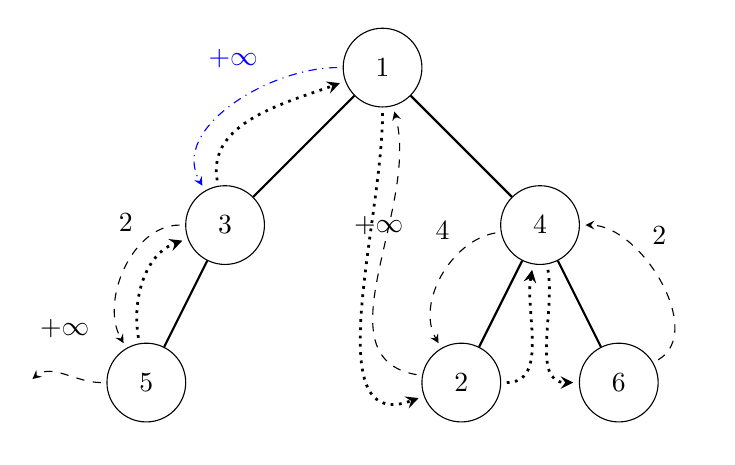
\begin{tikzpicture}[baseline=-2.25cm]
        \node[circle,draw,minimum size=1cm] (1) at (0,0)  {$1$};
        \node[circle,draw,minimum size=1cm] (2) at (-2,-2){$3$};
        \node[circle,draw,minimum size=1cm] (3) at (2,-2) {$4$};
        \node[circle,draw,minimum size=1cm] (4) at (-3,-4){$5$};
        \node[circle,draw,minimum size=1cm] (5) at (1,-4) {$2$};
        \node[circle,draw,minimum size=1cm] (6) at (3,-4) {$6$};
        % \node[label={7},circle,draw,minimum size=1cm] (7) at (3,-4) {$8$};
        % \node[label={8},circle,draw,minimum size=1cm] (8) at (-4,-6) {$4$};
        % \node[label={9},circle,draw,minimum size=1cm] (9) at (-2,-6) {$1$};
        \tikzstyle{filho}=[thick]
        \tikzstyle{pred}=[->, shorten >= 2pt, shorten <= 2pt,
        dashed, >=stealth]
        \tikzstyle{sucessor}=[->, shorten >= 2pt, shorten <= 2pt,
        dotted, >=stealth, line width=0.35mm]
        % \tikzstyle{p4}=[->, shorten >= 2pt, shorten <= 2pt, dotted, >=stealth]
        \draw[filho] (1) -- (2);
        \draw[filho] (1) -- (3);
        \draw[filho] (2) -- (4);
        \draw[filho] (3) -- (5);
        \draw[filho] (3) -- (6);
        \draw[pred] (6) edge[out=30,in=0]
        node[above=10pt] {$2$} (3);
        \draw[sucessor] (3) edge[out=280,in=180] (6);
        \draw[pred] (3) edge[out=190,in=120]
        node[above=10pt] {$4$} (5);
        \draw[sucessor] (5) edge[out=0,in=260] (3);
        \draw[pred] (5) edge[out=170,in=285]
        node[above=10pt] {$+\infty$} (1);
        \draw[sucessor] (1) edge[out=270,in=200] (5);
        \draw[pred, blue, dashdotted] (1) edge[out=180,in=120]
        node[blue, above=10pt] {$+\infty$} (2);
        \draw[sucessor] (2) edge[out=100,in=200] (1);
        \draw[pred] (2) edge[out=180,in=120]
        node[above=10pt] {$2$} (4);
        \draw[sucessor] (4) edge[out=100,in=200] (2);
        \draw[pred] (4) edge[out=180,in=40]
        node[above=10pt] {$+\infty$} (-4.5, -4);
    \end{tikzpicture}
    \begin{tabular}{|c|c|c|c|c|}
        \hline
        &       &       & $\now = 1.5$                \\
        $i$ & $x_0$ & $v$   & $\cert[i]$                  \\
        \hline
        $1$ & $6$   & $2$   & \textcolor{blue}{$+\infty$} \\

        $2$ & $3$   & $5$   & $+\infty$                   \\

        $3$ & $2$   & $1$   & $2$                         \\

        $4$ & $7$   & $4$   & $4$                         \\

        $5$ & $-2$  & $3$   & $+\infty$                   \\

        $6$ & $14$  & $0.5$ & $2$                         \\
        \hline
    \end{tabular}
    \caption[ABB após chamar \textsc{delete}]{Após chamar
        {\normalfont \textsc{delete}$(7)$} na árvore da Figura~\ref{fig:abb:insert}, o
    elemento $7$ foi retirado da árvore, a lista ligada foi
    ajustada, o certificado do seu sucessor, o elemento $1$, foi
    atualizado e o certificado do elemento $7$ foi destruído.}
    \label{fig:abb:delete}
\end{figure}

\begin{figure}[htb]
    \centering
    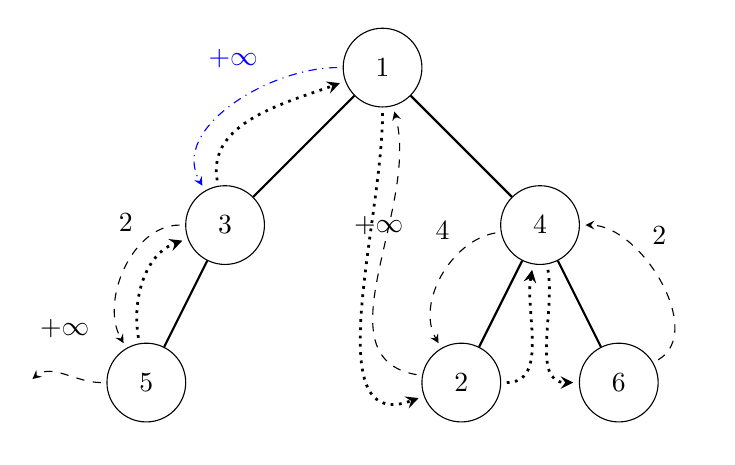
\begin{tikzpicture}[baseline=-2.25cm]
        \node[circle,draw,minimum size=1cm] (1) at (0,0)  {$1$};
        \node[circle,draw,minimum size=1cm] (2) at (-2,-2){$3$};
        \node[circle,draw,minimum size=1cm] (3) at (2,-2) {$4$};
        \node[circle,draw,minimum size=1cm] (4) at (-3,-4){$5$};
        \node[circle,draw,minimum size=1cm] (5) at (1,-4) {$2$};
        \node[circle,draw,minimum size=1cm] (6) at (3,-4) {$6$};
        % \node[label={7},circle,draw,minimum size=1cm] (7) at (3,-4) {$8$};
        % \node[label={8},circle,draw,minimum size=1cm] (8) at (-4,-6) {$4$};
        % \node[label={9},circle,draw,minimum size=1cm] (9) at (-2,-6) {$1$};
        \tikzstyle{filho}=[thick]
        \tikzstyle{pred}=[->, shorten >= 2pt, shorten <= 2pt,
        dashed, >=stealth]
        \tikzstyle{sucessor}=[->, shorten >= 2pt, shorten <= 2pt,
        dotted, >=stealth, line width=0.35mm]
        % \tikzstyle{p4}=[->, shorten >= 2pt, shorten <= 2pt, dotted, >=stealth]
        \draw[filho] (1) -- (2);
        \draw[filho] (1) -- (3);
        \draw[filho] (2) -- (4);
        \draw[filho] (3) -- (5);
        \draw[filho] (3) -- (6);
        \draw[pred] (6) edge[out=30,in=0]
        node[above=10pt] {$2$} (3);
        \draw[sucessor] (3) edge[out=280,in=180] (6);
        \draw[pred] (3) edge[out=190,in=120]
        node[above=10pt] {$4$} (5);
        \draw[sucessor] (5) edge[out=0,in=260] (3);
        \draw[pred] (5) edge[out=170,in=285]
        node[above=10pt] {$+\infty$} (1);
        \draw[sucessor] (1) edge[out=270,in=200] (5);
        \draw[pred, blue, dashdotted] (1) edge[out=180,in=120]
        node[blue, above=10pt] {$+\infty$} (2);
        \draw[sucessor] (2) edge[out=100,in=200] (1);
        \draw[pred] (2) edge[out=180,in=120]
        node[above=10pt] {$2$} (4);
        \draw[sucessor] (4) edge[out=100,in=200] (2);
        \draw[pred] (4) edge[out=180,in=40]
        node[above=10pt] {$+\infty$} (-4.5, -4);
    \end{tikzpicture}
    \begin{tabular}{|c|c|c|c|c|}
        \hline
        &       &       & $\now = 1.5$                \\
        $i$ & $x_0$ & $v$   & $\cert[i]$                  \\
        \hline
        $1$ & $6$   & $2$   & \textcolor{blue}{$+\infty$} \\

        $2$ & $3$   & $5$   & $+\infty$                   \\

        $3$ & $2$   & $1$   & $2$                         \\

        $4$ & $7$   & $4$   & $4$                         \\

        $5$ & $-2$  & $3$   & $+\infty$                   \\

        $6$ & $14$  & $0.5$ & $2$                         \\
        \hline
    \end{tabular}
    \caption[ABB após chamar \textsc{delete}]{Após chamar
        {\normalfont \textsc{delete}$(7)$} na árvore da Figura~\ref{fig:abb:insert}, o
    elemento $7$ foi retirado da árvore, a lista ligada foi
    ajustada, o certificado do seu sucessor, o elemento $1$, foi
    atualizado e o certificado do elemento $7$ foi destruído.}
    \label{fig:abb:delete}
\end{figure}

\begin{algorithm}
    \caption{Função \textsc{deleteTourn}.} \label{torneioi:deletetourn}
    \begin{algorithmic}[1]
        \Function{deleteTourn}{$e$}
            \State $i \leftarrow $ \Call{substitute}{$e$}
            \State $k \leftarrow 2\cdot \floor{i/2} + ((i + 1)\mod2)$
            \While{$i > 1$}
                \If{\Call{compare}{$k, i$}}
                    \State $i \leftrightarrow k$
                \EndIf
                \State $\torneio[\floor{i/2}] \leftarrow \torneio[i]$
                \State $\torneio[k].\lastmatch \leftarrow k$
                \State \Call{update}{$\torneio[k]$}
                \State $i \leftarrow \floor{i/2}$
                \State $k \leftarrow 2\cdot \floor{i/2} + ((i + 1)\mod2)$
                \Comment{adversário}
            \EndWhile
            \State $\torneio[1].\lastmatch \leftarrow 1$
                \State \Call{update}{$\torneio[1]$}
        \EndFunction
    \end{algorithmic}
\end{algorithm}
